\chapter{Localisation}

This chapter focuses on robot localisation and simultaneous localisation and mapping (SLAM) in a simulated environment. Localisation is achieved through odometry computations to determine the robot's position and orientation, while Graph SLAM builds on this foundation to simultaneously construct a map and localise the robot within it.

\section{Localisation Using Odometry}

Robot localisation involves computing its position and orientation using wheel encoder readings, a method known as odometry. The robot calculates the distance traveled by each wheel, determining the forward movement as:

\[
\Delta_{\text{center}} = \frac{\Delta_{\text{left}} + \Delta_{\text{right}}}{2}
\]

and the change in orientation as:

\[
\Delta_{\theta} = \frac{\Delta_{\text{right}} - \Delta_{\text{left}}}{\text{wheel base}}
\]

Using these values, the robot updates its global position and orientation at each step of the simulation. The updated coordinates are given by:

\[
x_{\text{new}} = x_{\text{old}} + \Delta_{\text{center}} \cdot \cos(\theta_{\text{old}})
\]

\[
y_{\text{new}} = y_{\text{old}} + \Delta_{\text{center}} \cdot \sin(\theta_{\text{old}})
\]

\[
\theta_{\text{new}} = \theta_{\text{old}} + \Delta_{\theta}
\]

The system continuously monitors the encoder values during each simulation step, ensuring real-time refinement of the robot's position and orientation. By leveraging these calculations, the robot maintains an accurate understanding of its location within the environment, which is essential for precise movement and navigation.

In this project, we initially set out to implement SLAM for the TurtleBot3 in the Webots simulation environment but realised our implementation was limited to localisation on a predetermined map rather than full SLAM. The TurtleBot3 was configured with motors for continuous movement, enabling exploration and data collection, and equipped with a LIDAR sensor for 360\degree{} obstacle detection. Encoders tracked wheel rotations, and odometry calculations used differential drive kinematics to update the robot's position and orientation. Localisation was achieved by updating the robot’s position based on encoder data and interpreting LIDAR data relative to a predefined rectangular map with fixed dimensions. This predefined knowledge of the environment meant that the implementation did not fully achieve SLAM, which requires both simultaneous mapping and localisation in an unknown environment. The robot updated its position and visualised its progress on the predetermined map in real-time, with periodic visualisations and debugging ensuring accuracy. Challenges, such as maintaining proper updates and sensor configuration, were addressed systematically.




\begin{figure}[H]
    \centering
    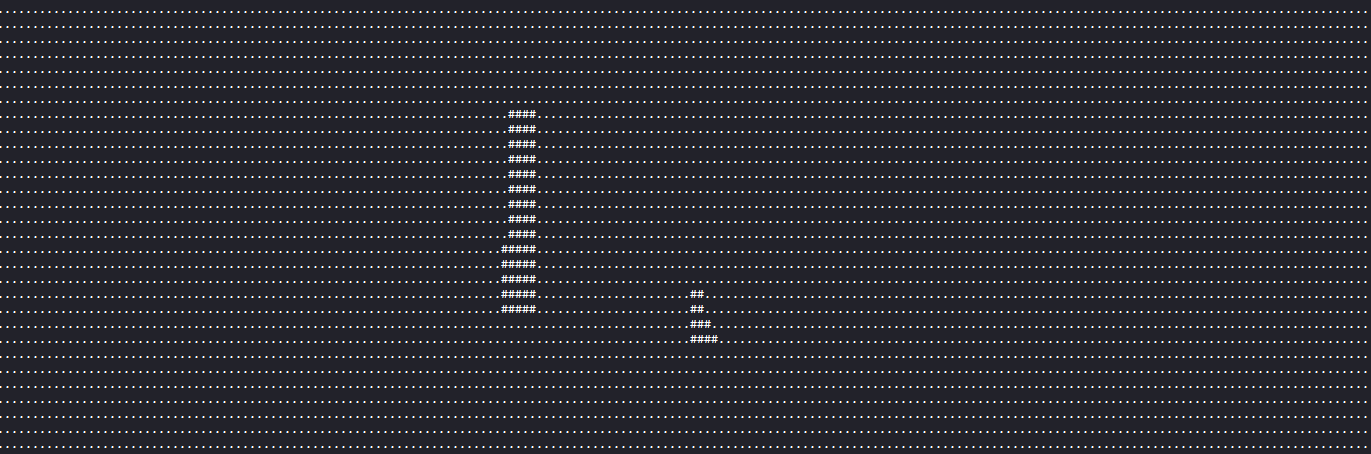
\includegraphics[width=1.0\linewidth]{midpoint_report/assets/images/localisation/map.png}
    \caption{A 2-D map depicting the location of the robot in its environment}
    \label{fig: map}
\end{figure}

\section{Graph SLAM}

Graph SLAM builds upon localisation by simultaneously constructing a map and localising the robot within it. The steps involved are outlined below:

\subsection{Create the Initial Graph Using Odometry}

The robot’s pose is updated using odometry as:
\[
x_{t} = x_{i} + \Delta s \cos(\theta_{i}),
\]
\[
y_{t} = y_{i} + \Delta s \sin(\theta_{i}),
\]
\[
\theta_{t} = \theta_{i} + \Delta \theta
\]
where \(\Delta s\) is the distance traveled.

The edge \(e_{ij}\) is represented as:
\[
e_{ij} =
\begin{bmatrix}
    \Delta x \\
    \Delta y \\
    \Delta \theta
\end{bmatrix}.
\]

\subsection{Loop Closure}

When the robot recognises a previously visited landmark, an additional edge is added between non-consecutive poses \(x_{i}\) and \(x_{j}\) where \(j \neq i + 1\). This edge is based on sensor measurements, not odometry:
\[
e_{ij} = \begin{bmatrix}
    \Delta x_{ij}\\
    \Delta y_{ij}\\
    \Delta \theta_{ij}
\end{bmatrix}.
\]

\subsection{Defining the Error Function/Residual}

\[
e_{ij} =
\begin{bmatrix}
    x_{j} - (x_{i} + \Delta x_{ij}) \\
    y_{j} - (y_{i} + \Delta y_{ij}) \\
    \theta_{j} - (\theta_{i} + \Delta \theta_{ij})
\end{bmatrix}.
\]
Here, \(x_{j}, y_{j}, \theta_{j}\) are the current noisy estimates, and \(x_{i} + \Delta x_{ij}, y_{i} + \Delta y_{ij}, \theta_{i} + \Delta \theta_{ij}\) are the expected values for pose \(j\).

\subsection{Objective Function/Sum of Squared Errors}

\[
f(x) = \sum_{(i,j) \in \text{edges}} e_{ij}(x_{i}, x_{j})^{T} \Omega_{ij} e_{ij}(x_{i}, x_{j}),
\]
where \(\Omega_{ij}\) is the information matrix. It measures the confidence in measurements, with examples like:
\[
\Omega_{ij} =
\begin{bmatrix}
    \omega_x & 0 & 0 \\
    0 & \omega_y & 0 \\
    0 & 0 & \omega_\theta
\end{bmatrix},
\]
where \(\omega_x, \omega_y, \omega_\theta\) are weighted confidences.

\subsection{Gauss-Newton Optimization}

\begin{enumerate}
    \item Linearise using Taylor expansion:
    \[
e_{ij}(x_{i}, x_{j}) \approx e_{ij}(x_{i0}, x_{j0}) + J_{ij}(x_{i} - x_{i0}),
    \]
    where \(J_{ij} = \frac{\partial e_{ij}}{\partial x}\bigg|_{x=x_{0}}\).

    \item Substitute into the objective function and expand:
\[
f(x) \approx \sum_{(i,j) \in \text{edges}} \left(
\begin{aligned}
& e_{ij}(x_{i0}, x_{j0})^{T} \Omega_{ij} e_{ij}(x_{i0}, x_{j0}) \\
& + 2 e_{ij}(x_{i0}, x_{j0})^{T} \Omega_{ij} J_{ij} (x - x_0) \\
& + (x - x_0)^{T} J_{ij}^{T} \Omega_{ij} J_{ij} (x - x_0)
\end{aligned}
\right).
\]





    \item Solve the normal equations:
    \[
H \Delta x = -g,
    \]
    where
    \[
H = \sum_{(i,j) \in \text{edges}} J_{ij}^{T} \Omega_{ij} J_{ij}, \quad g = \sum_{(i,j) \in \text{edges}} J_{ij}^{T} \Omega_{ij} e_{ij}(x_{i0}, x_{j0}).
    \]

    \item Use Cholesky decomposition for efficiency:
    \[
H = L L^{T},
    \]
    solve \(L y = -g\), then \(L^{T} \Delta x = y\).

    \item Update:
    \[
x \leftarrow x + \Delta x.
    \]

    Repeat until convergence.
\end
